\documentclass[11pt,a4paper]{article}
\usepackage[utf8]{inputenc}
\usepackage[T1]{fontenc}
\IfFileExists{lmodern.sty}{\usepackage{lmodern}}{}
\IfFileExists{french.ldf}{\usepackage[french]{babel}}{\usepackage[english]{babel}}
\usepackage{amsmath,amssymb,amsfonts,amsthm}
\usepackage{geometry}
\geometry{top=2cm, bottom=2cm, left=2.2cm, right=2.2cm}
\usepackage{booktabs,array,multirow}
\usepackage{enumitem}
\usepackage{xcolor}
\usepackage{tcolorbox}
\tcbuselibrary{skins,breakable}
\usepackage{tikz}
\usetikzlibrary{arrows.meta,positioning,shapes.geometric,calc}
\usepackage[colorlinks=true,linkcolor=blue!60!black]{hyperref}
\newtcolorbox{propbox}[1]{colback=blue!5!white,colframe=blue!75!black,fonttitle=\bfseries,title={#1},breakable,boxrule=0.8pt}
\newtcolorbox{rembox}[1]{colback=orange!5!white,colframe=orange!80!black,fonttitle=\bfseries,title={#1},breakable,boxrule=0.8pt}
\newtcolorbox{verifbox}{colback=green!4!white,colframe=green!45!black,fonttitle=\bfseries,title=Vérification algorithmique (Python),breakable,boxrule=0.6pt}
\newcommand{\Xt}{\tilde{X}}
\newcommand{\Yt}{\tilde{Y}}
\setlength{\parindent}{0pt}
\setlength{\parskip}{4pt}
\title{\textbf{Université Akli Mohand Oulhadj -- Bouira}\\
\large Master Recherche Opérationnelle (RO) -- 2025/2026\\
\Large \textbf{Théorie des Jeux : Solution Détaillée du TD n$^\circ$2}\\
\large Jeux non coopératifs -- Équilibres de Nash}
\author{\textbf{Référence de cours :} Chapitre 1 (notions, domination)\\ Chapitre 2 (jeux non coopératifs, équilibre de Nash)}
\date{}

\begin{document}
\maketitle
\hrule
\vspace{0.4cm}

\begin{propbox}{Rappels du cours (Chapitre 2, pages 3--7)}
Un jeu sous forme normale est $J=\langle I,X,f\rangle$ avec $I=\{1,\dots,n\}$, $X=\prod_i X_i$, $f=(f_1,\dots,f_n)$, $f_i:X\to\mathbb{R}$ gain du joueur $i$. Notation : $(t_i,x_{I-i})=(x_1,\dots,x_{i-1},t_i,x_{i+1},\dots,x_n)$.

\textbf{Équilibre de Nash :} $x^*\in X$ tel que
\[
\forall i\in I,\ \forall x_i\in X_i,\qquad f_i(x_i,x^*_{I-i})\le f_i(x^*_i,x^*_{I-i}).
\]
\emph{Aucun joueur ne peut augmenter strictement son gain en changeant seul de stratégie.}

\textbf{Méthode pratique (jeu bimatriciel) :} pour chaque colonne, on souligne le meilleur gain du joueur 1 ; pour chaque ligne, le meilleur gain du joueur 2. Les cases doublement soulignées sont les équilibres de Nash en stratégies pures.
\end{propbox}

%=====================================================================
\section*{Exercice 1 : La chasse au cerf}

Joueur 1 en ligne, joueur 2 en colonne, stratégies $C$ (cerf) et $L$ (lapin) :
\[
\begin{array}{c|cc}
 & C & L\\\hline
C & (10,10) & (0,8)\\
L & (8,0) & (7,7)
\end{array}
\]

\subsection*{1. Équilibres de Nash}
\paragraph{Test de chaque issue (définition).}
\begin{itemize}
\item $(C,C)$ : J1 dévie vers $L$ : $8<10$ ; J2 dévie vers $L$ : $8<10$. Aucune déviation profitable : \textbf{équilibre}.
\item $(C,L)$ : J1 dévie vers $L$ : $7>0$. \textbf{Pas un équilibre.}
\item $(L,C)$ : J2 dévie vers $L$ : $7>0$. \textbf{Pas un équilibre.}
\item $(L,L)$ : J1 dévie vers $C$ : $0<7$ ; J2 dévie vers $C$ : $0<7$. \textbf{Équilibre.}
\end{itemize}
\paragraph{Méthode des meilleures réponses.} $R_1(C)=C$, $R_1(L)=L$, $R_2(C)=C$, $R_2(L)=L$. Les intersections des graphes sont $(C,C)$ et $(L,L)$.
\[
\boxed{\begin{array}{c}\text{Équilibres de Nash en stratégies pures :}\\ (C,C) \text{ de gains } (10,10) \quad\text{et}\quad (L,L) \text{ de gains } (7,7).\end{array}}
\]

\paragraph{Complément : équilibre en stratégies mixtes.} Soit $q$ la probabilité que J2 joue $C$. J1 est indifférent entre $C$ et $L$ si
\[
10q+0(1-q)=8q+7(1-q)\iff 10q=7+q\iff q=\tfrac79.
\]
Par symétrie, J1 joue $C$ avec $p=\frac79$. Gain espéré de chacun : $10\cdot\frac79=\frac{70}{9}\approx7{,}78$. Il y a donc trois équilibres au total (deux purs, un mixte).

\subsection*{2. Issue Pareto-optimale}
Une issue est Pareto-optimale s'il n'existe pas d'autre issue qui améliore le gain d'un joueur sans diminuer celui de l'autre. Ici $(10,10)$ est supérieure ou égale composante par composante à $(0,8)$, $(8,0)$ et $(7,7)$, avec une inégalité stricte.
\[
\boxed{(C,C) \text{ est l'unique issue Pareto-optimale.}}
\]
\begin{rembox}{Interprétation}
$(L,L)$ est un équilibre mais n'est pas Pareto-optimal : c'est l'équilibre « prudent » (chasser seul garantit $7$ ou $8$, alors que viser le cerf risque $0$). C'est la même remarque que dans le cours (p.~7) : une issue meilleure pour les deux joueurs n'est atteinte que s'il y a coordination entre eux.
\end{rembox}

%=====================================================================
\section*{Exercice 2 : Jeu de la poule mouillée (« chicken »)}
\[
\begin{array}{c|cc}
 & s_1 & s_2\\\hline
t_1 & (-3,-3) & (2,-1)\\
t_2 & (-1,2) & (0,0)
\end{array}
\]
\begin{itemize}
\item $(t_1,s_1)$ : J1 dévie vers $t_2$ : $-1>-3$. Non.
\item $(t_1,s_2)$ : J1 dévie : $0<2$ ; J2 dévie vers $s_1$ : $-3<-1$. \textbf{Équilibre.}
\item $(t_2,s_1)$ : J1 dévie vers $t_1$ : $-3<-1$ ; J2 dévie vers $s_2$ : $0<2$. \textbf{Équilibre.}
\item $(t_2,s_2)$ : J1 dévie vers $t_1$ : $2>0$. Non.
\end{itemize}
\[
\boxed{\text{Équilibres de Nash purs : } (t_1,s_2) \text{ de gains } (2,-1) \text{ et } (t_2,s_1) \text{ de gains } (-1,2).}
\]
\paragraph{Complément mixte.} J2 joue $s_1$ avec probabilité $q$ ; J1 indifférent si $-3q+2(1-q)=-q\iff 2-5q=-q\iff q=\frac12$. Par symétrie $p=\frac12$. Gain espéré : $\frac12(-3)+\frac12(2)=-\frac12$ pour chacun.

\textbf{Pas de stratégie dominée} : pour J1, $t_1$ est meilleure contre $s_2$ ($2>0$) mais pire contre $s_1$ ($-3<-1$). L'élimination itérée ne résout pas ce jeu, contrairement à l'exercice suivant.

%=====================================================================
\section*{Exercice 3 : Exploitation d'une prairie commune}

\subsection*{1. Forme normale}
Chaque agriculteur $i$ choisit son nombre de vaches $x_i\in X_i=\{0,1,2\}$. Si le total est $N=x_1+x_2\ge1$, chaque vache rapporte $r(N)$ avec $r(1)=8$, $r(2)=5$, $r(3)=3$, $r(4)=2$. Le gain est
\[
f_i(x_1,x_2)=x_i\,r(x_1+x_2)\qquad(\text{et } f_i=0 \text{ si } x_i=0).
\]
$J=\langle I=\{1,2\},\ X_1=X_2=\{0,1,2\},\ f_1,f_2\rangle$ :
\[
\begin{array}{c|ccc}
x_1\backslash x_2 & 0 & 1 & 2\\\hline
0 & (0,0) & (0,8) & (0,10)\\
1 & (8,0) & (5,5) & (3,6)\\
2 & (10,0) & (6,3) & (4,4)
\end{array}
\]
(Par exemple $(1,2)$ : $N=3$, $r=3$, gains $1\cdot3=3$ et $2\cdot3=6$.)

\subsection*{2. Élimination itérée des stratégies dominées}
Gains de J1 par ligne : $L_0=(0,0,0)$, $L_1=(8,5,3)$, $L_2=(10,6,4)$. On a
\[
L_2=(10,6,4)>(8,5,3)=L_1>(0,0,0)=L_0 \quad\text{composante par composante, strictement.}
\]
Donc « 2 vaches » \textbf{domine strictement} $0$ et $1$ : c'est une stratégie \textbf{strictement dominante} pour J1. Le jeu est symétrique : il en va de même pour J2. Après élimination de $0$ et $1$ pour chacun, il reste l'issue unique
\[
\boxed{(2,2),\ \text{gains } (4,4),\ \text{unique équilibre de Nash.}}
\]
\textbf{Analogie :} c'est le \textbf{dilemme du prisonnier} (et la « tragédie des biens communs ») : chacun a intérêt individuellement à surexploiter, et l'équilibre $(4,4)$ est moins bon pour tous que $(1,1)$ qui donne $(5,5)$.

\subsection*{3. Optimum social et contrat}
\paragraph{Optimum social} (maximisation de $f_1+f_2$) :
\[
\begin{array}{c|ccc}
 & 0 & 1 & 2\\\hline
0 & 0 & 8 & 10\\
1 & 8 & 10 & 9\\
2 & 10 & 9 & 8
\end{array}
\]
Le maximum $10$ est atteint en $(1,1)$, $(0,2)$ et $(2,0)$ (soit 2 vaches au total). L'allocation optimale \emph{équitable} est $(1,1)$ avec $(5,5)$.

\paragraph{Contrat.} Chacun s'engage à ne mettre qu'une vache ; une tierce partie inflige une sanction $S$ à celui qui en met deux. Les gains deviennent (on retire $S$ à celui qui joue $2$) :
\[
\begin{array}{c|ccc}
 & 0 & 1 & 2\\\hline
0 & (0,0) & (0,8) & (0,10-S)\\
1 & (8,0) & (5,5) & (3,6-S)\\
2 & (10-S,0) & (6-S,3) & (4-S,4-S)
\end{array}
\]
\begin{itemize}
\item $(1,1)$ est un équilibre de Nash $\iff$ la déviation vers $2$ n'est pas profitable : $6-S<5\iff S>1$ (déviation vers $0$ : $0<5$, jamais profitable).
\item Si $S>1$, $(2,2)$ cesse d'être un équilibre : $4-S<3$. On vérifie qu'aucune autre issue n'est un équilibre (le joueur qui a $0$ vache gagne strictement à en mettre une). Pour $S>1$, \textbf{$(1,1)$ est l'unique équilibre de Nash}.
\item Pour $S=1$ : déviations à gain égal, $(2,2)$ reste un équilibre : insuffisant.
\item Si l'on veut que respecter le contrat soit \emph{strictement dominant} (garanti quel que soit l'autre) : $8>10-S$, $5>6-S$, $3>4-S$, c'est-à-dire $S>2$.
\end{itemize}
\[
\boxed{S>1 \text{ suffit pour que } (1,1) \text{ soit l'unique équilibre ; } S>2 \text{ le rend strictement dominant.}}
\]

%=====================================================================
\section*{Exercice 4 : Jeu continu sur $[-1,1]^2$}
$X_1=X_2=[-1,1]$, $f_1(x_1,x_2)=-x_1^2+2x_1x_2$, $f_2(x_1,x_2)=-x_2^2+2x_1x_2$.

\subsection*{1. Conditions du théorème de Nash}
\begin{propbox}{Théorème d'existence de Nash (forme utilisée en TD)}
Si pour tout $i$ : $X_i$ est un compact convexe non vide de $\mathbb{R}^{k}$, $f_i$ est continue sur $X$, et $x_i\mapsto f_i(x_i,x_{I-i})$ est concave (ou quasi-concave) pour tout $x_{I-i}$, alors $J$ admet au moins un équilibre de Nash. (C'est l'analogue, pour $n$ joueurs, du théorème de Von Neumann du chapitre 2.)
\end{propbox}
\begin{enumerate}[label=(\alph*)]
\item $[-1,1]$ est fermé, borné (compact), convexe et non vide. \checkmark
\item $f_1,f_2$ sont polynomiales, donc continues sur $[-1,1]^2$. \checkmark
\item $\frac{\partial^2 f_1}{\partial x_1^2}=-2<0$ et $\frac{\partial^2 f_2}{\partial x_2^2}=-2<0$ : $f_1$ est concave en $x_1$, $f_2$ concave en $x_2$. \checkmark
\end{enumerate}
\[
\boxed{\text{Les conditions sont vérifiées : il existe au moins un équilibre de Nash.}}
\]

\subsection*{2. Ensemble des issues}
L'ensemble des issues est $X=X_1\times X_2=[-1,1]^2$, le carré représenté ci-dessous ; on y trace aussi les meilleures réponses (question 3).
\begin{center}
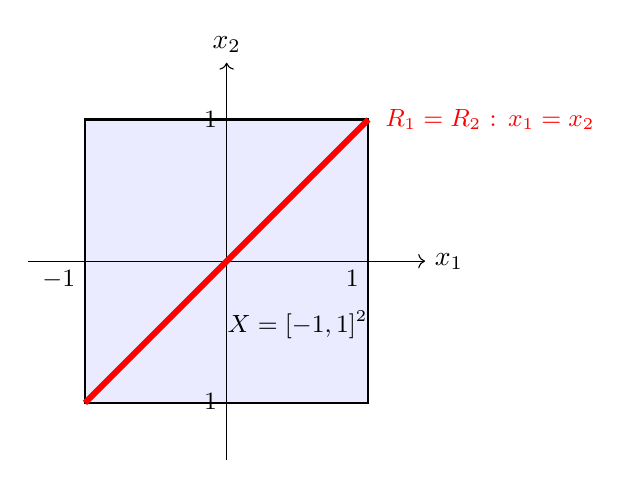
\begin{tikzpicture}[scale=1.8]
\fill[blue!8] (-1,-1) rectangle (1,1);
\draw[thick] (-1,-1) rectangle (1,1);
\draw[->] (-1.4,0)--(1.4,0) node[right]{$x_1$};
\draw[->] (0,-1.4)--(0,1.4) node[above]{$x_2$};
\node[below left] at (1,0) {\small $1$}; \node[below left] at (-1,0) {\small $-1$};
\node[left] at (0,1) {\small $1$}; \node[left] at (0,-1) {\small $-1$};
\draw[red,line width=2.2pt] (-1,-1)--(1,1);
\node[red,right] at (1.05,1.0) {\small $R_1=R_2$ : $x_1=x_2$};
\node at (0.5,-0.45) {\small $X=[-1,1]^2$};
\end{tikzpicture}
\end{center}

\subsection*{3. Équilibres de Nash}
\textbf{Meilleure réponse de J1.} À $x_2$ fixé, $\varphi(x_1)=-x_1^2+2x_1x_2$ est une parabole concave de sommet
\[
\varphi'(x_1)=-2x_1+2x_2=0\iff x_1=x_2\in[-1,1].
\]
Le sommet est dans l'intervalle, donc $R_1(x_2)=\{x_2\}$ (unique par stricte concavité). Par symétrie $R_2(x_1)=\{x_1\}$.

\textbf{Intersection des meilleures réponses.} $x^*$ est un équilibre $\iff x_1^*=x_2^*$ et $x_2^*=x_1^*$ :
\[
\boxed{\mathcal{E}_{Nash}=\{(t,t)\ :\ t\in[-1,1]\}\quad\text{(toute la diagonale du carré)},\qquad f_1(t,t)=f_2(t,t)=t^2.}
\]
\textbf{Vérification par la définition.} $f_1(x_1,t)=-x_1^2+2x_1t=t^2-(x_1-t)^2\le t^2=f_1(t,t)$ ; de même pour J2. \checkmark
\begin{rembox}{Remarque}
Il y a une infinité d'équilibres. Les équilibres $(1,1)$ et $(-1,-1)$, de gains $(1,1)$, sont Pareto-supérieurs à tous les autres (par exemple $(0,0)$ donne $(0,0)$) : comme dans l'exercice 1, les équilibres de Nash ne sont pas tous Pareto-optimaux.
\end{rembox}

%=====================================================================
\section*{Exercice 5 : Duopole de Cournot}
$X_1=X_2=[0,+\infty[$, $f_1(x_1,x_2)=[p-(x_1+x_2)]x_1$, $f_2(x_1,x_2)=[p-(x_1+x_2)]x_2$, avec $p>0$.

\subsection*{1. Meilleure réponse $R_i$}
Par définition, $R_1(x_2)=\{x_1^*\in X_1:\ f_1(x_1^*,x_2)\ge f_1(x_1,x_2),\ \forall x_1\in X_1\}$.

À $x_2\ge0$ fixé, $\varphi(x_1)=(p-x_2)x_1-x_1^2$ est strictement concave ($\varphi''=-2$), avec $\varphi'(x_1)=p-x_2-2x_1$.
\begin{itemize}
\item Si $x_2<p$ : $\varphi'(x_1)=0\iff x_1=\frac{p-x_2}{2}>0$, point admissible, c'est le maximum.
\item Si $x_2\ge p$ : $\varphi'(x_1)=p-x_2-2x_1<0$ pour tout $x_1>0$, $\varphi$ est décroissante sur $[0,+\infty[$ : maximum en $x_1=0$.
\end{itemize}
\[
\boxed{R_1(x_2)=\max\Big(0,\ \frac{p-x_2}{2}\Big)=\begin{cases}\dfrac{p-x_2}{2} & \text{si } 0\le x_2< p\\[2mm] 0 & \text{si } x_2\ge p\end{cases},\qquad R_2(x_1)=\max\Big(0,\ \frac{p-x_1}{2}\Big).}
\]

\subsection*{2. Représentation graphique}
\begin{center}
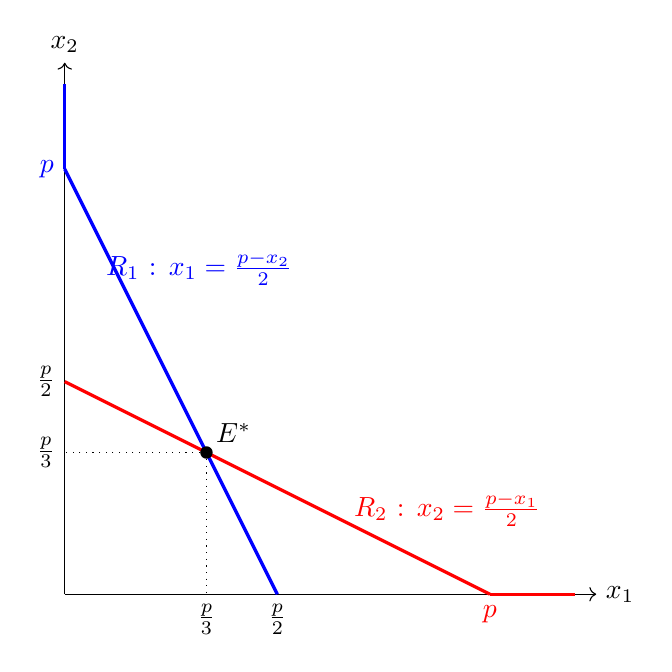
\begin{tikzpicture}[scale=0.9]
\draw[->] (0,0)--(7.5,0) node[right]{$x_1$};
\draw[->] (0,0)--(0,7.5) node[above]{$x_2$};
\draw[blue,very thick] (3,0)--(0,6) node[left]{$p$};
\draw[blue,very thick] (0,6)--(0,7.2);
\node[blue] at (1.9,4.6) {$R_1$ : $x_1=\frac{p-x_2}{2}$};
\draw[red,very thick] (0,3)--(6,0) node[below]{$p$};
\draw[red,very thick] (6,0)--(7.2,0);
\node[red] at (5.4,1.2) {$R_2$ : $x_2=\frac{p-x_1}{2}$};
\node[below] at (3,0) {$\frac p2$}; \node[left] at (0,3) {$\frac p2$};
\fill (2,2) circle (2.5pt);
\draw[dotted] (2,2)--(2,0) node[below]{$\frac p3$};
\draw[dotted] (2,2)--(0,2) node[left]{$\frac p3$};
\node[above right] at (2,2) {$E^*$};
\end{tikzpicture}
\end{center}
$R_1$ est le segment joignant $(0,p)$ à $(\frac p2,0)$ (prolongé par $x_1=0$ pour $x_2\ge p$) ; $R_2$ est le segment joignant $(0,\frac p2)$ à $(p,0)$ (prolongé par $x_2=0$ pour $x_1\ge p$).

\subsection*{3. Équilibre de Nash}
L'équilibre est l'intersection des graphes de $R_1$ et $R_2$ (DM2, Partie 1). Pour une solution intérieure :
\[
\begin{cases}2x_1+x_2=p\\ x_1+2x_2=p\end{cases}\ \Rightarrow\ x_1^*=x_2^*=\frac p3.
\]
Les points de bord ne conviennent pas : si $x_1=0$ alors $x_2\in R_2(0)=\{\frac p2\}$, mais $R_1(\frac p2)=\{\frac p4\}\ne\{0\}$.
\[
\boxed{x^*=\Big(\frac p3,\frac p3\Big),\quad \text{prix } p-\frac{2p}{3}=\frac p3,\quad f_1^*=f_2^*=\frac{p^2}{9}.}
\]
\begin{rembox}{Remarque (comparaison avec l'optimum collectif)}
Si les firmes s'entendaient (monopole partagé), elles maximiseraient $(p-Q)Q$ avec $Q=\frac p2$, d'où un profit total $\frac{p^2}{4}>\frac{2p^2}{9}$. L'équilibre de Nash n'est donc pas Pareto-optimal pour les firmes : même structure que la prairie commune.
\end{rembox}

\vspace{0.4cm}
\begin{verifbox}
Recontrôlé dans \texttt{verification\_TDJ.py} : énumération exhaustive des équilibres purs (Ex.~1, 2, 3), formules d'indifférence ($p=q=\frac79$ et $\frac12$), frontière de Pareto, matrice de la prairie, optimum social, et équilibres avec sanction pour $S=1$ (insuffisant), $S=1{,}5$ et $S=2{,}5$ ; calcul symbolique (\texttt{sympy}) des meilleures réponses des Ex.~4 et~5, vérification numérique sur grille que toute la diagonale est d'équilibre, et $x^*=(\frac p3,\frac p3)$, profit $\frac{p^2}{9}$.
\end{verifbox}

\end{document}
